%        File: paper.tex
%     Created: Tue Nov 09 06:00 PM 2010 E
% Last Change: Tue Nov 09 06:00 PM 2010 E
%
\documentclass[a4paper,twocolumn]{article}
\usepackage{graphicx}
\usepackage{amsmath}

\title{The Navier-Stokes Equations:\\ The Last Unsolved Classical Mechanics Problem}
\author{Andrew Gibiansky}
\date{\today}

\begin{document}
\maketitle

\section{Introduction}

\subsection{Classical Mechanics}

Classical mechanics, the father of physics and perhaps of scientific thought, was initially developed in the 1600s by the famous natural philosophers (the codename for 'physicists') of the 17th century such as Isaac Newton building on the data and observations of astronomers including Tycho Brahe, Galileo, and Johannes Kepler. Classical mechanics concerns itself with the mathematical description of the motion of physical bodies, tying together the concepts of force, momentum, velocity, and energy to describe the behaviour of macroscopic objects [1]. Though it was developed nearly 400 years ago, many of the basic tenets of classical mechanics hold for common situations (excluding microscopic particle dynamics, high-velocity motion, and large-scale mechanics). Classical mechanics holds accurately for scales from 1 picometer ($10^{-12}$ meters) to $10^{30}$ meters. Due to its consistent success, classical mechanics has been widely studied by physicists and mathematicians alike. Even though it must rely on quantum mechanics for small-scale motion and special relativity for high-velocity travel, it is considered a mostly complete and solved set of theories. However, there is still one problem in classical mechanics which remains unsolved: the solution - in fact, whether a solution is guaranteed to exist - to the general case of the Navier-Stokes equations for fluid dynamics is unknown.

\subsection{Fluid Dynamics and the Navier-Stokes Equations}

The Navier-Stokes equations, developed by Claude-Louis Navier and George Gabriel Stokes in 1822, are equations which can be used to determine the velocity vector field that applies to a fluid, given some initial conditions. They arise from the application of Newton's second law in combination with a fluid stress (due to viscosity) and a pressure term. For almost all real situations, they result in a system of nonlinear partial differential equations; however, with certain simplifications (such as 1-dimensional motion) they can sometimes be reduced to linear differential equations. Usually, however, they remain nonlinear, which makes them difficult or impossible to solve; this is what causes the turbulence and unpredictability in their results. 



\section{Derivation of the Navier-Stokes Equations}

The Navier-Stokes equations can be derived from the basic conservation and continuity equations applied to properties of fluids. In order to derive the equations of fluid motion, we must first derive the continuity equation (which dictates conditions under which things are conserved), apply the equation to conservation of mass and momentum, and finally combine the conservation equations with a physical understanding of what a fluid is.

\subsection{Continuity Equation}

The basic continuity equation is an equation which describes the change of an intensive property $L$. An intensive property is something which is independent of the amount of material you have. For instance, temperature would be an intensive property; heat would be the corresponding extensive property. The volume $\Omega$ is assumed to be of any form; its bounding surface area is referred to as $\partial\Omega$. The continuity equation derived can later be applied to mass and momentum.

\subsubsection{Reynold's Transport Theorem}

The first basic assumption is that of Reynold's Transport Theorem, usually symbolized as follows:
\[\frac{d}{dt}\int_\Omega L \;dV = - \int_{\partial\Omega} L\vec v \cdot \vec n\;dA - \int_\Omega Q\; dV.\]
The left hand side of the equation denotes the rate of change of the property $L$ contained inside the volume $\Omega$. The right hand side is the sum of two terms:
\begin{itemize}
    \item A flux term, $\int_{\partial\Omega} L\vec v \cdot \vec n\;dA$, which indicates how much of the property $L$ is leaving the volume by flowing over the boundary $\partial\Omega$
    \item A sink term, $\int_\Omega Q\; dV$, which describes how much of the property $L$ is leaving the volume due to sinks or sources inside the boundary
\end{itemize}
In plain English, this equation states that the change in the total amount of a property is due to how much flows out through the volume boundary as well as how much is lost or gained through sources or sinks inside the boundary.

For example, if the intensive property we are dealing with is temperature, the equations states that the total change in heat is the sum of the heat flux (heat flowing out of the boundary) and the heat sources or sinks in the medium. If the intensive property we're dealing with is density, then the equation is simply a statement of conservation of mass: the change in mass is the sum of what leaves the boundary and what appears within it; no mass is left unaccounted for.

\subsubsection{Divergence Theorem}

The Divergence Theorem allows the flux term of the above equation to be rexpressed as a volume integral. By the Divergence Theorem,
\[\int_{\partial\Omega} L\vec v\cdot\vec n\;dA = \int_{\Omega} \nabla\cdot(L\vec v)\;dV.\]
Therefore, we can now rewrite our previous equation as 
\[\frac{d}{dt}\int_\Omega L \;dV = - \int_{\Omega} \nabla\cdot(L\vec v) + Q\; dV.\]

\subsubsection{Resulting Equation}

Leibniz's Rule states that 
\[\frac{d}{dx}\int_a^b f(x,y)\;dy = \int_a^b \frac{d}{dx}f(x,y)\;dy.\]
Thus, after applying this rule to the previous equation, we find that
\[\int_\Omega \frac{d}{dt}L \;dV = - \int_{\Omega} \nabla\cdot(L\vec v) + Q\; dV.\]
Equivalently, 
\[\int_\Omega \frac{d}{dt}L +  \nabla\cdot(L \vec v) + Q\;dV = 0.\]
This relation applies to any control volume $\Omega$; the only way the above equality remains true for all control volumes is if the integrand itself is zero. Thus, we arrive at the general form of the continuity equation
\[\frac{dL}{dt} + \nabla\cdot(L\vec v) + Q = 0.\]

\subsection{Conservation of Mass}

Applying the continuity equation to density (the intensive property equivalent to mass), we obtain
\[\frac{d\rho}{dt} + \nabla\cdot(\rho\vec v) + Q = 0.\]
This is the same as conservation of mass because we are operating with a constant control volume $\Omega$. With no sources or sinks of mass $(Q=0)$,
\[\frac{d\rho}{dt} + \nabla\cdot(\rho\vec v) = 0.\]
This is the equation of conversation of mass.\\\\
In some cases, such as when we have a pipe pumping fluid in or out of the system inside the control volume, we might not want to assume that $Q=0$; however, for the general case, we make the assumption that mass is not added or removed from the system. \\

However, in certain cases it is useful to simplify it further. For an incompressible fluid, the density is constant. Setting the derivative of density equal to zero and dividing through by a constant $\rho$, we obtain the simplest form of the equation
\[\nabla\cdot\vec v = 0.\]

\subsection{Material Derivative}

A necessary concept for the derivation of the conservation of momentum equations is that of the material derivative. A normal derivative is the rate of change of of an intensive property at a point. For instance, the value $\frac{dT}{dt}$ could be the rate of change of temperature at a point $(x,y)$. However, a material derivative is the rate of change of an intensive property on a particle in a velocity field. It must incorporate two things:
\begin{itemize}
    \item Rate of change of the property, $\frac{dL}{dt}$
    \item Change in position of othe particle in the velocity field $\vec v$
\end{itemize}
Logically speaking, therefore, the material derivative can be defined as
\[\frac{Du}{Dt} = \frac{du}{dt} + (\vec v \cdot \nabla)u.\]
The expression
\[(\vec v \cdot \nabla)u\]
represents the directional derivative of $u$ in the direction of the velocity $\vec v$. 


\subsection{Conversation of Momentum}

Although the most rigorous derivation of the conservation of momentum equations also stems from the general form continuity equation formed above, a quicker and nearly as rigorous derivation can be done using Newton's laws and an application of the chain rule. Basic physics dictates that
\[\vec F = m\vec a.\]
Allowing for the body force $\vec F=\vec b$ and substituting density for mass, we get a similar equation
\[\vec b = \rho \frac{d}{dt} \vec v(x,y,z,t).\]
Note that we can substitute density for mass because we are, as before, operating with a fixed control volume and infinitesimal fluid parcels. \\

The body force $\vec b$ is a force that acts throughout the body of fluid (as opposed to, say, a shear force, which acts parallel to a plane). \\

Applying the chain rule to the derivative of velocity, we get
\[\vec b = \rho(\frac{\partial \vec v}{\partial t} + \frac{\partial \vec v}{\partial x}\frac{\partial x}{\partial t}  + \frac{\partial \vec v}{\partial y}\frac{\partial y}{\partial t} + \frac{\partial \vec v}{\partial z}\frac{\partial z}{\partial t}).\]
Equivalently,
\[\vec b = \rho(\frac{\partial \vec v}{\partial t} + \vec v \cdot \nabla \vec v).\]
Substituting the value in parentheses for the definition of a material derivative, we obtain our final equation of
\[\rho\frac{D\vec v}{Dt} = \vec b.\]

\subsection{Equations of Motion}

The conservations equations derived above, in addition to a few assumptions about the forces and the behaviour of fluids, lead to the equations of motionfor fluids. 

We assume that the body force on the fluid parcels is due to two components, fluid stresses and other, external forces. 
\[\vec b = \nabla \cdot \sigma + \vec f.\]
Here, $\sigma$ is the stress tensor, and $\vec f$ represents external forces. Intuitively, the fluid stress is represtented as the divergence of the stress tensor because the divergence is the extent to which the tensor acts like a sink or source; in other words, the divergence of the tensor results in a momentum source or sink, also known as a force. For many applications it is sufficient to say that $\vec f$ is composed only of gravity, but for now we will leave the equation in its most general form. 

\subsection{Stresses}

The equations of motion depend on the stress tensor $\sigma$. The tensor can be represented as 
\[\sigma =  \left( \begin{array}{ccc}
    \sigma_{xx} &  \tau_{xy} & \tau_{xz} \\
\tau_{yx} &  \sigma_{yy} & \tau_{yz} \\
\tau_{zx} &  \tau_{zy} & \sigma_{zz}
\end{array} \right).\]
A tensor is a generalization of the concept of the higher-order quantity; a vector is represented as a first order tensor, a matrix as a second order tensor, a 3D matrix is a third order tensor, and so on.
\pagebreak

\begin{figure}[htb]
    \centering
    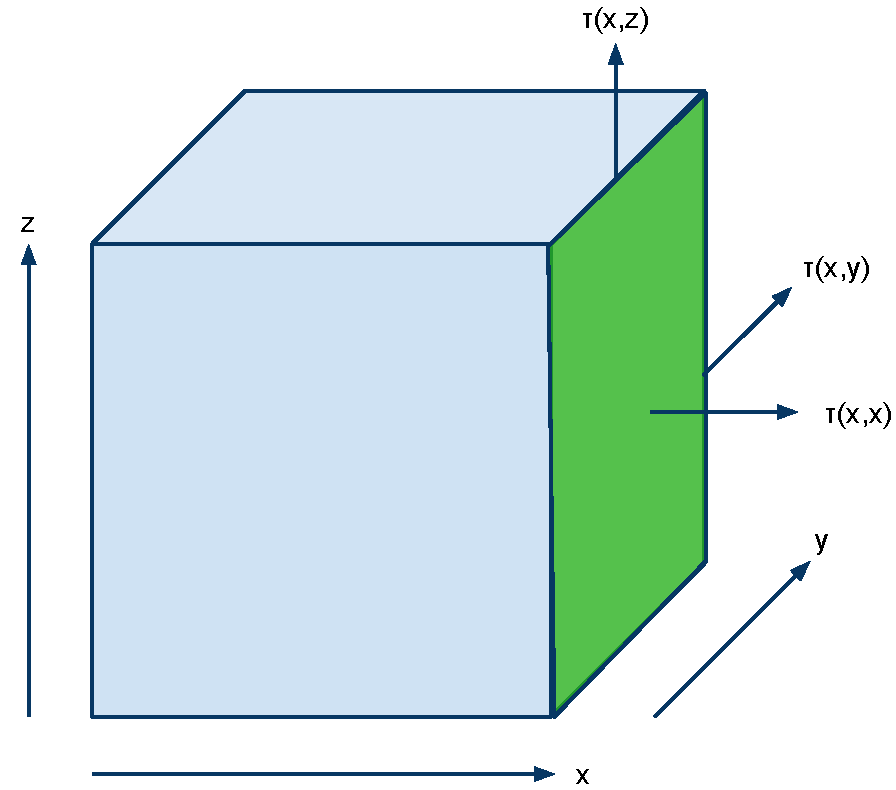
\includegraphics[width=200pt]{Stresses.pdf}
    \caption{Illustrated shear and normal stress tensors}
\end{figure}

$\tau_{ab}$ indicates the stress on the plane perpendicular to the axis $a$ and in the direction of the axis $b$. Thus, when $a=b$, $\tau_{ab}$ would be a normal stress, while otherwise it would be a shear stress. For future reference, note that the divergence of a tensor is a vector where each component is the divergence of the respective column vector of the tensor.

\subsection{General Form of the Navier-Stokes Equation}

The stress tensor $\sigma$ denoted above is often divided into two terms of interest in the general form of the Navier-Stokes equation. The two terms are the volumetric stress tensor, which tends to change the volume of the body, and the stress deviator tensor, which tends to deform the body. The volumetric stress tensor represents the force which sets the volume of the body (namely, the pressure forces). The stress deviator tensor represents the forces which determine body deformation and movement, and is composed of the shear stresses on the fluid. Thus, $\sigma$ is broken down into

\[\sigma =  \left( \begin{array}{ccc}
    \sigma_{xx} &  \tau_{xy} & \tau_{xz} \\
\tau_{yx} &  \sigma_{yy} & \tau_{yz} \\
\tau_{zx} &  \tau_{zy} & \sigma_{zz}
\end{array} \right) = \] \[ = -\left( \begin{array}{ccc}
    p &  0 & 0 \\
0 &  p & 0 \\
0 &  0 & p 
\end{array} \right) +\]\[+ \left( \begin{array}{ccc}
    \sigma_{xx} + p &  \tau_{xy} & \tau_{xz} \\
\tau_{yx} &  \sigma_{yy} + p & \tau_{yz} \\
\tau_{zx} &  \tau_{zy} & \sigma_{zz} + p
\end{array} \right).\]
Denoting the stress deviator tensor as $T$, we can make the substitution
\[\sigma = -pI + T.\]\\

Substituting this into the previous equation, we arrive at the most general form of the Navier-Stokes equation:
\[\rho\frac{D\vec v}{Dt} = -\nabla p + \nabla \cdot T + \vec f.\]

Although this is the general form of the Navier-Stokes equation, it cannot be applied until it has been more specified. First off, depending on the type of fluid, an expression must be determined for the stress tensor $T$; secondly, if the fluid is not assumed to be incompressible, an equation of state and an equation dictating conservation of energy are necessary.

\subsection{Physical Explanation of the Navier-Stokes Equation}
The Navier-Stokes equation makes a surprising amount of intuitive sense given the complexity of what it is modeling. The left hand side of the equation,
\[\rho\frac{D\vec v}{Dt},\]
is the force on each fluid particle. The equation states that the force is composed of three terms:
\begin{itemize}
    \item $-\nabla p$: A pressure term (also known as the volumetric stress tensor) which prevents motion due to normal stresses. The fluid presses against itself and keeps it from shrinking in volume.
    \item $\nabla\cdot T$: A stress term (known as the stress deviator tensor) which causes motion due to horizontal friction and shear stresses. The shear stress causes turbulence and viscous flows - if you drag your hand through a liquid, you will note that the moving liquid also causes nearby liquid to start moving in the same direction. Turbulence is the result of the shear stress.
    \item $\vec f$: The force term which is acting on every single fluid particle.
\end{itemize}

This intuitively explains turblent flows and some common scenarios. For example, if water is sitting in a cup, the force (gravity) $\rho g$ is equal to the pressure term because $\frac{d}{dz}(\rho g z) = \rho g.$ Thus, since gravity is equivalent to the pressure, the fluid will sit still, which is indeed what we observe when water is sitting in a cup.

\section{Navier-Stokes Fluids}
The general form Navier-Stokes equation derived above cannot be used in practice, as it has a number of unspecified elements. These are usually specific to the fluid which the equation is being applied to. A number of fluid models exist, varying the tensor $T$ and the equation of state (for compressible fluids). 

\subsection{Newtonian Fluids}
For simplicity of derivation, we will assume the Newtonian fluid is incompressible, though in truth many common fluids (such as air) are compressible, and the equations and methods have been thoroughly studied for compressible Newtonian fluids as well.

\subsubsection{Fluid Stress}
The basis for the Newtonian fluid equations is the assumption about the nature of the stress tensor. For a Newtonian Fluid, the stress is proportional to the rate of deformation (the change in velocity in the directions of the stress). In other words,
\[\tau_{ij} = \mu\left(\frac{\partial u_i}{\partial x_j} + \frac{\partial u_j}{\partial x_i}\right).\]

The proportionality constant $\mu$ is called the viscosity of the fluid, and defines how easily the fluid flows when subjected to body forces. 

\subsubsection{Stress Divergence}
The Navier-Stokes equation uses the divergence of stress, $\nabla\cdot T$. We can calculate the stress term
\[\nabla\cdot\sigma =  \mu \nabla\cdot\left( \begin{array}{ccc}
    \sigma_{xx} &  \tau_{xy} & \tau_{xz} \\
\tau_{yx} &  \sigma_{yy} & \tau_{yz} \\
\tau_{zx} &  \tau_{zy} & \sigma_{zz}
\end{array} \right) =\]\[= \mu\left( \begin{array}{ccc}
    2\frac{\partial u}{\partial x} & \frac{\partial u}{\partial y}+\frac{\partial v}{\partial x} & \frac{\partial u}{\partial z}+\frac{\partial w}{\partial x} \\
    \frac{\partial u}{\partial y}+\frac{\partial v}{\partial x} & 2\frac{\partial v}{\partial y} & \frac{\partial v}{\partial z} + \frac{\partial w}{\partial y} \\
    \frac{\partial u}{\partial z}+\frac{\partial w}{\partial x} & \frac{\partial v}{\partial z} + \frac{\partial w}{\partial y} & 2\frac{\partial w}{\partial z} 
\end{array}\right). \]

We can calculate the $x$ term of the divergence:
\begin{align*}
(\nabla\cdot\sigma)_i &= \mu\frac{\partial}{\partial x}(2\frac{\partial u}{\partial x}) + \frac{\partial}{\partial y}(\frac{\partial u}{\partial y}+\frac{\partial v}{\partial x}) + \frac{\partial}{\partial z}(\frac{\partial u}{\partial z}+\frac{\partial w}{\partial x}) = \\
&= \mu\frac{\partial^2 u}{\partial x^2} + \frac{\partial^2 u}{\partial y^2} + \frac{\partial^2 u}{\partial z^2} + \frac{\partial^2 u}{\partial x^2} + \frac{\partial^2 v}{\partial x \partial y} + \frac{\partial^2 w}{\partial x \partial z} = \\
&= \mu\nabla^2 u + \mu\frac{\partial}{\partial x}(\frac{\partial u}{\partial x} + \frac{\partial v}{\partial y} + \frac{\partial w}{\partial z}) = \\
&= \mu\nabla^2 u + \mu\frac{\partial}{\partial x}(\nabla\cdot v) 
&= \nabla^2 u + 0 = \\
&= \mu\nabla^2 u.\\
\end{align*}

We can extend this to the other divergence terms, so we can replace the divergence with a vector Laplacian:
\[\nabla\cdot T = \mu \nabla^2 v.\]

\subsubsection{Newtonian Fluid Equation}
Without making any assumptions about the form of the body force $f$, the final equation for an incompressible Newtonian fluid would be
\[\rho\frac{Dv}{Dt} = -\nabla p + \mu \nabla^2 v + f.\]

\subsection{Non-Newtonian Fluids}

Though Newtonian fluids are the most commonly encountered and the most studied of all fluid models, a few others exist as well. 

\subsubsection{Bingham Plastics}
A Bingham Plastic is similar to a Newtonian fluid, but differs in one key aspect: while Newtonian fluids will start motion as soon as some shear stress is applied, a Bingham plastic fluid is able to resist stress until the stress passes a certain yield threshold. Afterwards, it will act the same as a Newtonian fluid. Some examples of Bingham plastics include toothpaste and clay. 

\subsubsection{Power-law Fluids}
Power-law fluids differ from Newtonian fluids in that the stress in a power-law fluid is raised to an exponent, $n$, called the flow behaviour index. While Newtonian fluids follow the equation
\[\tau = \mu \left( \frac{\partial u}{\partial y} \right),\]
power-law fluids model stress according to the equation
\[\tau = \mu \left( \frac{\partial u}{\partial y} \right)^n.\]


Thus, Newtonian fluids are a subset of power-law fluids, since a Newtonian fluid is a power-law fluid with $n=1$. When $n<1$, the material is termed a pseudoplastic; pseudoplastics decrease in viscosity as the shear stress increases. Common examples of pseudoplastics include lava, whipped cream, blood, and many polymer solutions. If $n>1$, the material is termed a dilatant; dilatants are rare, and have an increasing viscosity with increasing shear stress. They tend to act in very non-intuitive manners. For instance, YouTube videos demonstrate oobleck (a mixture of cornstarch and water) becoming nearly solid when put under stress, but remaining liquid otherwise; this would allow someone to run across a pool of oobleck, but sink if they stood still on it.

\subsection{Simulations}
Due to the complex nature of the Navier-Stokes equations, analytical solutions range from difficult to practically impossible, so the most common way to make use of the Navier-Stokes equations is through simulation and approximation. A number of simulation methods exist, and in the next section, we will examine one of the algorithms often used in computer graphics and interactive applications.

\section{Smoothed Particle Hydrodynamics}
One of the most researched and most used methods for fluid simulations, especially in interactive applications, is a particle-based approach known as Smoothed Particle Hydrodynamics (SPH). SPH is, at the most basic level, an attempt to discretize the Navier-Stokes equations. In addition to the fluid particles themselves, a smoothing function (called the smoothing kernel) is used which spreads the properties of each particle over a continuum. In fact, SPH is often called ``an interpolation method for particle systems.'' We will now derive and demonstrate the use of SPH for modeling a simple incompressible Newtonian fluid.

\subsection{Smoothing Kernels and Basis of SPH}
Since SPH is essentially an interpolation method for particle systems, one of the key ideas behind it is the ability to evaluate a scalar quantity in any point in space, even though the quantity only truly has a value at the discrete particles. \\

In order to evaluate a quantity $A$ at a point $\vec r$, we use the following equation:
\[A(\vec r) = \sum_j m_j\frac{A_j}{\rho_j}\cdot W(|\vec r - \vec r_j|, h).\]

This is a weighted summation of all the particles around the point. $A_j$ is the value of $A$ at the particle, $m_j$ is the mass of the particle, $\rho_j$ is the density of the particle, and $W(|\vec r - \vec r_j|, h)$ is the weighting factor, and $h$ is the maximum distance. The function $W$ is also called the \emph{smoothing kernel}, because it smoothes the particle values throughout continuous space. \\


    The smoothing function $W$ has a few notable properties. First of all, the function should decrease as the distance increases; this is only logical, since the points nearby should have more influence than those far away. Second of all, the kernel should evaluate to 0 at distances equal to or greater than $h$. Finally, the smoothing kernel should be normalized. A normalized smoothing kernel satisfies the equation
\[\int W(|\vec r|, h) dr = 1.\]

\subsubsection{Derivatives of Quantities}
The Navier-Stokes equations often require calculating the first or second derivatives of various quantities. This is particularly easy in SPH, because the derivative of a quantity is
\[\frac{\partial}{\partial \vec r} A(\vec r) = \frac{\partial}{\partial \vec r} \sum_j m_j\frac{A_j}{\rho_j}\cdot W(|\vec r - \vec r_j|, h).\]
Equivalently,
\[\frac{\partial}{\partial \vec r} A(\vec r) = \sum_j m_j\frac{A_j}{\rho_j}\cdot \frac{\partial}{\partial \vec r} W(|\vec r - \vec r_j|, h).\]
Thus,
\[\nabla A(\vec r) = \sum_j m_j\frac{A_j}{\rho_j}\cdot \nabla W(|\vec r - \vec r_j|, h)\]
and
\[\nabla^2 A(\vec r) = \sum_j m_j\frac{A_j}{\rho_j}\cdot \nabla^2 W(|\vec r - \vec r_j|, h).\]

\subsubsection{Calculating Density}
As you may have noticed, the equation for the SPH value of a scalar quantity includes both a mass and a density term. This is because each particle represents a small volume $V_i = \frac{m_i}{\rho_i}$. The Navier-Stokes equations for an incompressible fluid (such as water) require that the density term is constant; however, due to the nature of SPH, maintaining a constant density is very difficult. Since in many applications accuracy is less important than realism and speed, we ignore the requirement that density is constant. We can later compensate for that by making the density restoring force (pressure) very strong. \\


Since density $\rho$ is non-constant, we may need to calculate density at a given position. Since density is yet another intensive property, we can apply the SPH equation above to get
\[\rho_j = \sum_j m_j \frac{\rho_j}{\rho_j} W(|\vec r - \vec r_j|, h) = \sum_j m_j W(|\vec r - \vec r_j|, h).\]

The problem of density is one of the biggest reasons not to use SPH for models which require precision or accuracy. SPH is meant to provide a realistic-looking fluid simulation, at the cost of ignoring certain requirements, such as symmetry, conservation of momentum, or constant density.

\subsection{Simulation}
The Navier-Stokes equations can now be applied to the SPH particles. We have two main equations. The first is the conservation of mass equation, 
\[\nabla\cdot\vec v = 0.\]


The second equation stems from the conservation of momentum, and states that 
\[\rho\frac{Dv}{Dt} = -\nabla p + \mu \nabla^2 v + f.\]

The first equation is guaranteed for particle systems, because we have a constant amount of particles, each with a constant mass. Therefore, the total mass remains constant, and we can ignore the first equation. The second equation dictates the motion of the particles. The left hand term is the change in momentum. Therefore, we can express the acceleration of each particle as
\[a_i = \frac{f_i}{\rho_i}\]
where $f_i$ is the sum of all the force terms on the right hand side. In order to be able to simulate the particle motion, we must express each of the force terms through a discrete summation.

\subsubsection{Force Terms: Pressure}
If we apply our SPH equation to pressure, we arrive at the equation
\[f^{pressure}_i = -\nabla p(\vec r) = -\sum m_j \frac{p_j}{\rho_j}\nabla W(|\vec r_i - \vec r_j|, h).\]


However, this isn't symmetric. Pressure should be symmetric, since every action should have an equal and opposite reaction; however, if we examine a 2-particle system, the pressure of particle $i$ depends on the pressure of particle $j$ and vice versa, so symmetry is not guaranteed in the general case. In order to rectify this, we can use a different pressure equation, which uses an average of particle pressures to ensure symmetry:
\[f^{pressure}_i = -\nabla p(\vec r) = -\sum m_j \frac{p_i + p_j}{2\rho_j}\nabla W(|\vec r_i - \vec r_j|, h).\]

We must also remember that the only state a particle keeps around is its mass, density, and velocity. Thus, we cannot just use pressure, we must calculate it. Using the ideal gas state equation, we can say that
\[p = k\rho.\]

In order to make the simulation more numerically stable, we can make pressure smaller by using the difference. Since the equation uses the gradient of pressure, the math is unchanged if we use the equation
\[p = k(\rho - \rho_o)\]
where $\rho_o$ is the rest density. By doing this substitution, we reduce the value of $p$, and thus decrease the effects of floating point rounding errors introduced by the computations.

\subsubsection{Force Terms: Viscosity}
Applying SPH principles to viscosity, we arrive at the equation
\[f^{viscosity}_i = \mu\nabla^2 v(\vec r_i) = \mu \sum m_j \frac{v_j}{\rho_j} \nabla^2 W(|\vec r_i - \vec r_j|, h).\]

However, we encounter the same problem as before, namely that the viscosity force is non-symmetric. We can resolve it in a similar manner, using the difference in velocities instead. The resulting equation takes the form of
\[f^{viscosity}_i = \mu \sum m_j \frac{v_j-v_i}{\rho_j} \nabla^2 W(|\vec r_i - \vec r_j|, h).\]

In physical terms, this equation states that a particle is accelerated in the direction that its environment is moving. Thinking about a floating particle in a stream of liquid, this makes sense.

\subsubsection{Force Terms: Surface Tension}
In a fluid, molecules experience intramolecular attraction forces. For a particle embedded inside the fluid, the force is evened out; however, for particles on the edge of the fluid, the force does cause an acceleration, and thus is non-negligible. Since each particle is the cause of the intramolecular attraction, we define another quantity (called ``color'' for convenience) such that $c$ is equal to 1 at every particle and 0 otherwise. Therefore, the equation that describes the SPH quantity for $c$ would be
\[c(\vec r) = \sum m_j \frac{c_j}{\rho_j} W(|\vec r_i - \vec r_j|, h).\]

Since $c$ is 1 at all particle locations, we can simplify this to say that
\[c(\vec r) = \sum m_j \frac{1}{\rho_j} W(|\vec r_i - \vec r_j|, h).\]

For physical reasons that are beyond the scope of this analysis, the surface tension force is equal to
\[f_{surface} = \sigma \kappa \vec n = -\sigma \nabla^2 c \frac{\vec n}{|\vec n|}.\]

We try to avoid calculating the force when $|\vec n|$ is small, because that causes problems because we are dividing by a small floating point number. We only calculate the surface tension force when $|\vec n|$ is greater than a given preset. The final equation for the surface tension force (when we calculate it) would be
\[f^{surface}_i = -\sigma \nabla^2 c \frac{\nabla c}{|\nabla c|}.\]

\subsubsection{Force Terms: External Forces}
External forces are simply applied to every particle as they would be to a normal mass. If a particle touches (or goes into) a solid object, it is reflected (pushed out with it's velocity vector reflected over the object normal vector).

\subsection{Smoothing Kernels}
The smoothing kernel functions are required to do the actual computations for simulation. The quality of simulation, as well as the speed and accuracy, highly depend on the choice of smoothing kernels. In the original SPH publication that investigated simulating fluids in real-time [2], the authors suggested the use of three different kernels for different things. Note that the smoothing kernels are piece-wise functions; the functions presented subsequently define the values of $W$ for $0 \leq r \leq h$. In other cases, $W = 0.$ Note that the following smoothing kernels are not normalized, and should be prior to use.

\subsubsection{General Smoothing Kernel}
The general smoothing kernel, used in all but two cases, is a sixth-degree polynomial with the equation
\[W_{g}(r, h) = \frac{315}{64\pi h^9} \left(h^2 - r^2\right)^3.\]

One of the benefits of this empirically designed kernel is that it uses $r^2$, which means that we never need to calculate $r$. Calculating $r$ would be an expensive operation, because it involves a square root; calculating $r^2$, however, involves only multiplication, and is thus much faster.

\subsubsection{Pressure Kernel}
For calculations involving pressure, the general kernel becomes zero when particles are very close together. This is not what fluids actually act like - in fact, as particles come closer together, they should repel more due to pressure instead of less. Thus, Desbrun [6] suggests a different smoothing kernel of the form
\[W_{p}( r, h) = \frac{15}{\pi h^6} \left(h - r\right)^3.\]

\subsubsection{Viscosity Kernel}
The final smoothing kernel we are using is specific to the viscosity term. If we were to use the general smoothing term for viscosity, two particles which are very close to each other could possibly increase in speed. This is incorrect, since viscosity is a friction force, which should not be increasing the energy in the system. Thus, the authors of the original fluid simulation SPH paper suggest using the kernel of
\[W_{v}(r, h) = -\frac{r^3}{2h^3} + \frac{r^2}{h^2} + \frac{h}{2r} - 1.\]

\section{Ongoing Research}
Although the Navier-Stokes equations were originally formulated nearly 200 years ago, fluid mechanics is a rapidly evolving field. The advent of computer technology has allowed physicists to accurately model the behaviour of fluids through iterative approximations of their behaviour, making the study of the Navier-Stokes equations still more important. Current research can be subdivided into two categories: one form of research is theoretical, seeking mathematical proof of the existence and smoothness of the solution to Navier-Stokes; the other branch of ongoing research is more focused on practical application of Navier-Stokes to real-world problems. Though in some cases the distinction is purely artificial, it is nonetheless useful in discussing the various topics currently being investigated.

\subsection{Theoretical Research}
The fundamental theoretical problem of Navier-Stokes is one of the seven Millenium Prize Problems. The Millenium Prize Problems are seven mathematical problems put forth by the Clay Mathematics Institute in the year 2000; the first person to offer a valid solution to any of the problems is promised a million-dollar reward. The problem of Navier-Stokes, as stated by the Clay Mathematics Institute, is as follows:\\


``\emph{Prove or give a counter-example of the following statement:}\\

In three space dimensions and time, given an initial velocity field, there exists a vector velocity and a scalar pressure field, which are both smooth and globally defined, that solve the Navier-Stokes equations.''\\


Though this statement itself has not been proven or indicated false, attempts at proof have come close. It is known that for Navier-Stokes in two dimensions, the solutions exist and are smooth. In addition, it is known that for low initial velocities, smooth solutions to 3-dimensional Navier-Stokes exist; however, for higher initial velocities, the existence of smooth solutions has not been proven. 

\subsection{Practical Research}
Though the mathematical problem posed by Navier-Stokes has not yet been resolved, computer-aided approximations are suitable for many purposes. From the design of aerodynamic aircraft to simulation of water for Pixar films, fluid simulations are highly used in industry. Much current research in the field of computational fluid dynamics (CFD) attempts to find faster or more-accurate approximation algorithms in order to make these simulations more useful still.

The methods used in CFD can be broken down into two categories: discretization models and turbulence models. Discretization models attempt to break the fluid into a discrete set of elements, and iteratively simulate the motion of the fluid through time using the Navier-Stokes equations. Turbulence models deal with turbulence, a chaotic type of fluid flow, which is nearly impossible to simulate as with the discretization models; instead, turbulence models attempt to track or obtain the value of specific properties of a fluid over time.

Though the basic equations used are the same, approximation methods often take different approaches, depending on their objective. Some methods, especially ones aimed towards very fast or interactive fluid simulation, use particle based modeling. A volume of fluid is subdivided into a finite number of particles, and each particle is subject to the velocity fields dictated by the Navier-Stokes equations as well as external forces. This model typically simplifies computation and implementation, and is commonly used in computer graphics and computer games. The particle nature is usually hidden by interpolating particle positions through a process called point splatting. Smoothed Particle Hydrodynamics, the method investigated in the previous section, falls under that category.  Other methods, however, use a three-dimensional grid (a ``mesh'') to model the fluid. The internals and boundaries are tracked through iterative Navier-Stokes approximations; the benefit of this method is a higher precision and higher flexibility in terms of interaction with other bodies, at the cost of computational speed. 

\end{document}


